\documentclass[10pt]{beamer}

\usepackage{stmaryrd}
\usepackage{beamerthemesplit}
\usepackage{xcolor}
\usepackage{hyperref}


\newcommand{\TSync}[0]{\ltimes}
\newcommand{\TWait}[0]{\rtimes}
\newcommand{\TTot}[0]{\bowtie}


\usetheme{Warsaw}
% per trasparenza su animazioni di blocchi
\setbeamercovered{dynamic}



\title{Rupos: Process analysis and ProM development}
\author{R.Bruni \and \alert{A.Corradini}  \and G.Ferrari 
  \and R.Guanciale  \and G.Spagnolo}
\date{\today \\ \textbf{\alert{RUPOS}}}

\begin{document}

\frame{\titlepage}

\section{Introduction}

\subsection{Summary}
\frame{
  \begin{block}{Strategy}
    \begin{itemize}
    \item Adopt and extend existing formal methods (Petri Nets)
    \item Integrate and extend existing sw-infrastructure (ProM)
    \item Methodology work-flow
      \begin{enumerate}
      \item Processes are provided as BPMN diagrams
      \item BPMN diagram is transformed into Petri Net
      \item Process Instance logs are processes by refined techniques
        available for PetriNet
      \item Analysis results are projected back to the starting BPMN model.
      \end{enumerate}
    \end{itemize}

  \end{block}
}


% VECCHIO PEZZO DElL'ARCHITETTURA
% \section{The The Process Monitoring platform}
% \subsection{Engineering efforts}

% %% \frame{
%%   \begin{block}{Overall architecture}
    
%%     \begin{itemize}
%%     \item \alert{ProM} an existing process analysis framework
%%     \item \alert{OpenSPCoop} the most adopted  open source SPCoop implementation
%%     \end{itemize}

%%   \end{block}
%%   \begin{center}
%%     \includegraphics[scale=0.30]{./fig/Platform01}
%%   \end{center}

%% }

%% \frame{
%%   \begin{block}{Overall architecture}
    
%%     \begin{itemize}
%%     \item \alert{ProM} an existing process analysis framework
%%     \item \alert{OpenSPCoop} the most adopted  open source SPCoop implementation
%%     \end{itemize}

%%   \end{block}
  
%%   \begin{center}
%%     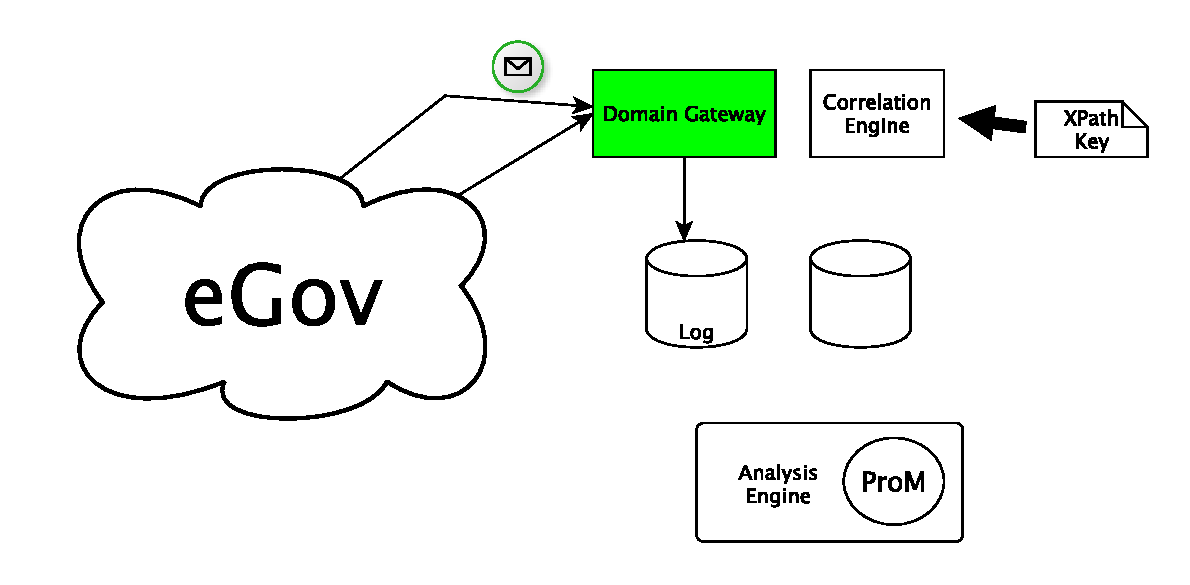
\includegraphics[scale=0.30]{./fig/Platform02}
%%   \end{center}

%%   \begin{itemize}
%%     \item eGov envelopes intercepted by Domain Gateway
%%     \item Domain Gateway stores message key information into the Log
%%       database
%%     %\item Domain Gateway performance are not affected by the analysis
%%     % \item <2-> Correlation engine groups SOAP request/response
%%     %   \begin{itemize}
%%     %     \item exploiting correlation sets (\alert{XPath})
%%     %     \item annotates process instances into log requests
%%     %     \item is externally triggered (e.g. cron/trigger)
%%     %   \end{itemize}
%%     % \item <3-> Analysis engine evaluates process metrics
%%     %   \begin{itemize}
%%     %     \item process definition stored in an external database (\alert{BPMN})
%%     %     \item process metrics stored into the log database
%%     %     \item is externally triggered (e.g. cron/trigger)
%%     %     \item fuffa su ProM
%%     %   \end{itemize}
%%   \end{itemize}
%% }

%% \frame{
%%   \begin{block}{Overall architecture}
    
%%     \begin{itemize}
%%     \item \alert{ProM} an existing process analysis framework
%%     \item \alert{OpenSPCoop} the most adopted  open source SPCoop implementation
%%     \end{itemize}

%%   \end{block}
  
%%   \begin{center}
%%     \includegraphics[scale=0.30]{./fig/Platform03}
%%   \end{center}

%%   \begin{itemize}
%%    \item eGov envelopes intercepted by Domain Gateway
%%     \item Domain Gateway stores message key information into the Log
%%       database
%%      \item Domain Gateway retrieves messages parts storing into the Log
%%       database
%%     %\item Domain Gateway performance are not affected by the analysis
%%     % \item <2-> Correlation engine groups SOAP request/response
%%     %   \begin{itemize}
%%     %     \item exploiting correlation sets (\alert{XPath})
%%     %     \item annotates process instances into log requests
%%     %     \item is externally triggered (e.g. cron/trigger)
%%     %   \end{itemize}
%%     % \item <3-> Analysis engine evaluates process metrics
%%     %   \begin{itemize}
%%     %     \item process definition stored in an external database (\alert{BPMN})
%%     %     \item process metrics stored into the log database
%%     %     \item is externally triggered (e.g. cron/trigger)
%%     %     \item fuffa su ProM
%%     %   \end{itemize}
%%   \end{itemize}
%% }

%% \frame{
%%   \begin{block}{Overall architecture}
    
%%     \begin{itemize}
%%     \item \alert{ProM} an existing process analysis framework
%%     \item \alert{OpenSPCoop} the most adopted  open source SPCoop implementation
%%     \end{itemize}

%%   \end{block}
  
%%   \begin{center}
%%     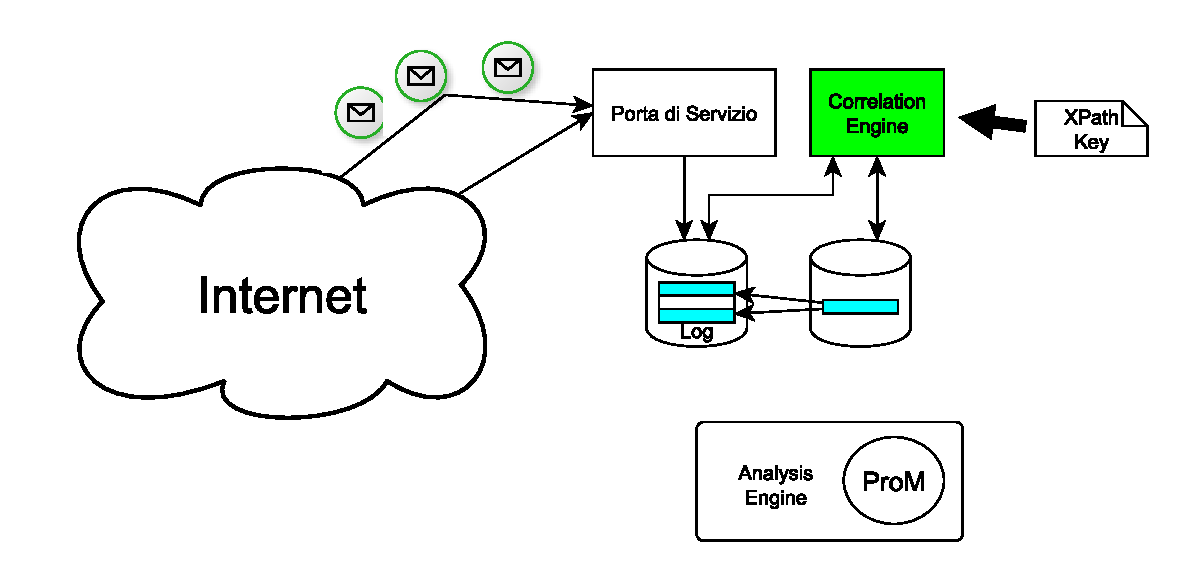
\includegraphics[scale=0.30]{./fig/Platform04}
%%   \end{center}

%%   \begin{itemize}
%%   \item eGov envelopes intercepted by Domain Gateway
%%     \item Domain Gateway stores message key information into the Log
%%       database
%%      \item Domain Gateway retrieves messages parts storing into the Log
%%       database
%%      \item Correlation engine groups SOAP request/response
%%        exploiting correlation sets (\alert{XPath})
%%      \item Service externally invoked (e.g. cron/trigger)
%%     % \item <3-> Analysis engine evaluates process metrics
%%     %   \begin{itemize}
%%     %     \item process definition stored in an external database (\alert{BPMN})
%%     %     \item process metrics stored into the log database
%%     %     \item is externally triggered (e.g. cron/trigger)
%%     %     \item fuffa su ProM
%%     %   \end{itemize}
%%   \end{itemize}
%% }

\begin{frame}{Architettura complessiva: integrazione di ProM in RUPOS}
  %% \begin{block}{}
    
  %%   \begin{itemize}
  %%   \item \alert{ProM} un framework per analisi di processi esistente
  %%   \item \alert{OpenSPCoop} the most adopted  open source SPCoop implementation
  %%   \end{itemize}

  %% \end{block}
  
  \begin{center}
    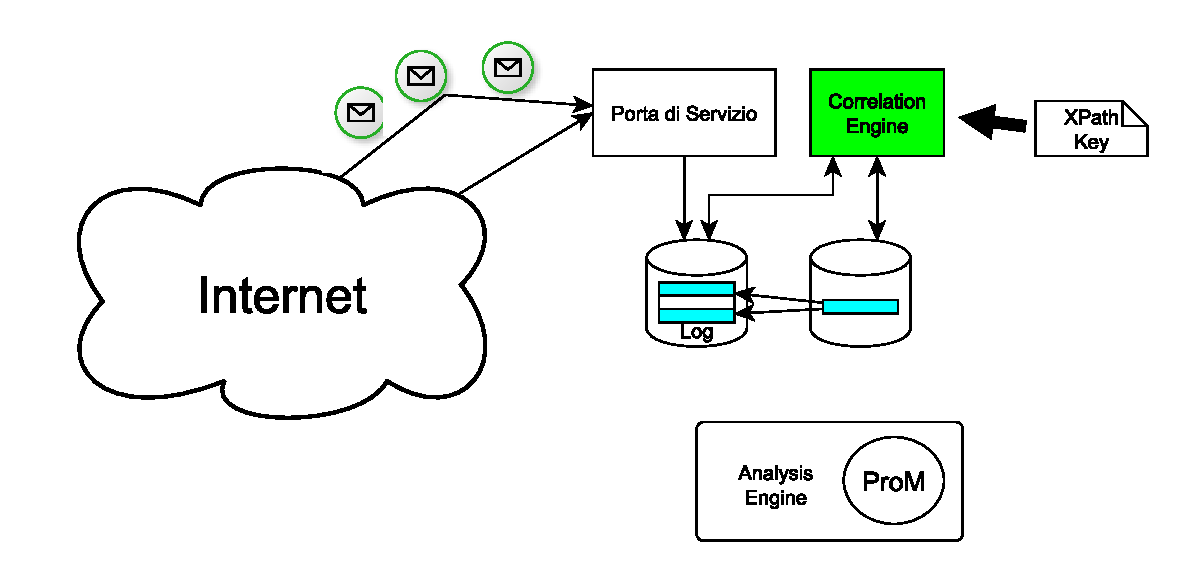
\includegraphics[scale=0.30]{./fig/Platform04}
  \end{center}

  \begin{itemize}
  \item I messaggi SOAP tra attori del processo vengono intercettati dalla Porta di Servizio (PdS)
    \item La PdS memorizza informazioni essenziali dei messaggi nel log
     \item La PdS estrae parti dei messaggi memorizzandoli nel database dei log
     \item Il Motore di Correlazione raggruppa i messaggi in istanze di processi usando ``correlation sets'' (\alert{XPath})
%     \item Service externally invoked (e.g. cron/trigger)
    \item I log di istanze di processi vengono trasformati in tracce di eventi corrispondenti a transizioni della Rete di Petri
%%  Gli eventi del log 

%% l framework di analisi calcola le metriche e annota il modello BPMN con i risultati
%    \item Service externally invoked (e.g. cron/trigger)
%    \item implements a context to integrate ProM into JBoss AS
  \end{itemize}
\end{frame}

%%% Local Variables: 
%%% mode: latex
%%% TeX-master: "main"
%%% End: 


\section{BPMN modeling}
\subsection{BPMN Example}
\frame{
  Rupos BPMN process example and its transformation
  
  \begin{center}
    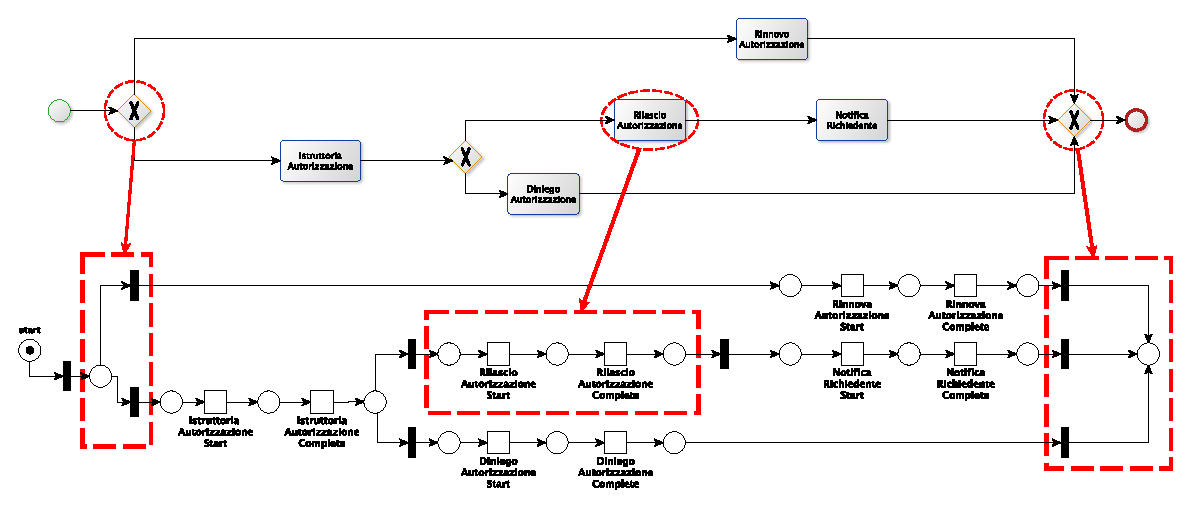
\includegraphics[scale=0.55]{./fig/BPMNandPN}
  \end{center}
}

\frame{
  \begin{block}{From SOAP messages to BPMN events}
  \begin{center}
  \begin{tiny}
    \begin{tabular}{|l|lll|}
      \hline
      \textbf{SOAP message} & \textbf{BPMN Event} &  &\\

      \hline
      richiestaAutorizzazione & AvvioProcedimento & AvvioProcedimento
      & \\
      request  &  start &  complete &\\

      \hline
      interrogaStatoAutorizzazione & RinnovaAutorizzazione &
      RinnovaAutorizzazione  & \\
      response[Rinnovo] & start & complete &\\

      \hline
      interrogaStatoAutorizzazione & RilascioAutorizzazione &
      RilascioAutorizzazione & \\
      response[Rilascio] & start & complete & \\

      \hline
      interrogaStatoAutorizzazione & RilascioAutorizzazione &
      NegaAutorizzazione & \\
      response[Nega] & start & complete & \\

      \hline
      richiestaParere & Parere &  & \\
      request & start & & \\

      \hline
      emissioneParere & Parere & ParereNegativo & ParereNegativo \\
      request[Negativo] & complete & start & complete\\

      \hline
      emissioneParere & Parere & ParerePositivo & ParerePositivo \\
      request[Positivo] & complete & start & complete\\

      \hline
      emissioneParere & Parere & ParereConRiserva & ParereConRiserva \\
      request[conRiserva] & complete & start & complete\\

      \hline
    \end{tabular}
  \end{tiny}
  \end{center}

  \end{block}

}

\section{Formal Analysis based on Petri nets}
\subsection{Adopted Petri Net techniques}
\frame{
  \begin{block}{Adopted Petri Net techniques}
    
    \begin{itemize}
      \item Process instance logs are ordered events
        (e.g. timestamp)
      \item Events are mapped to net transitions
      \item \alert{Log Replay}: replay a process instance log in a
        non-blocking way
        
        \begin{enumerate}
          \item Put a token in the start place
          \item Extract head event of the log
          \item fire the corresponding transition
            \begin{itemize}
              \item if the transition is not enabled
              artificially create the missing tokens
            \end{itemize}
        \end{enumerate}
      \item Metrics
        \begin{itemize}
          \item Number of missing/remaining token for each places/transition
          \item Number of edge traversal
          \item sojourn/waiting/synchronization time for each place
        \end{itemize}
    \end{itemize}

  \end{block}
}

% \frame{
  \begin{block}{Log-replay examples}
    Trace log $(A, 1s), (B, 2s), (C, 4s), (D, 8s)$ 
  \end{block}
  \begin{center}
    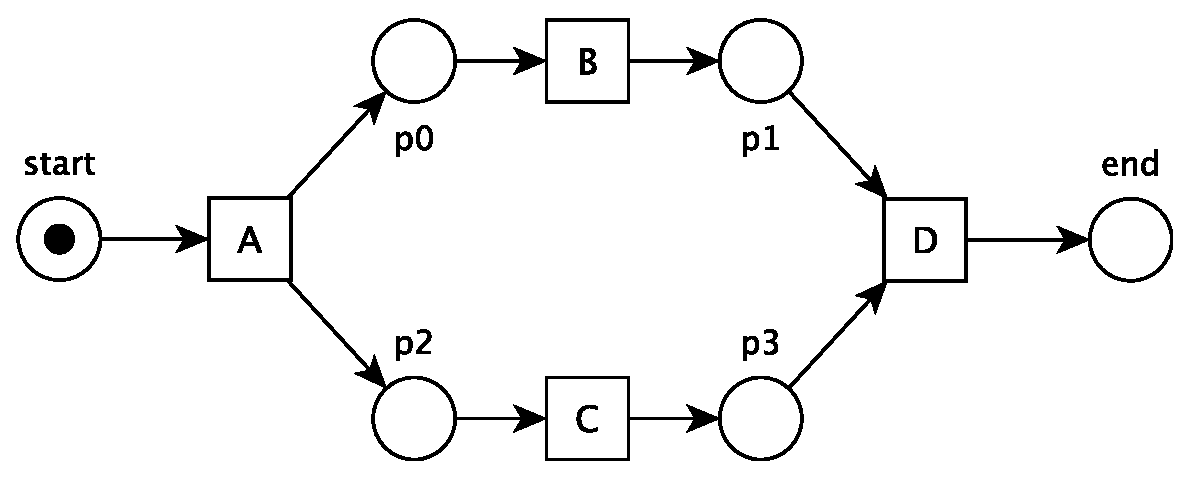
\includegraphics[scale=0.30]{./fig/LogReplay1a}
  \end{center}
  \begin {block}{Measures}
    \begin{tabular}{cc}
    \end{tabular}
  \end{block}
}
\frame{
  \begin{block}{Log-replay examples}
    Trace log $\alert{(A, 1s)}, (B, 2s), (C, 4s), (D, 8s)$ 
  \end{block}
  \begin{center}
    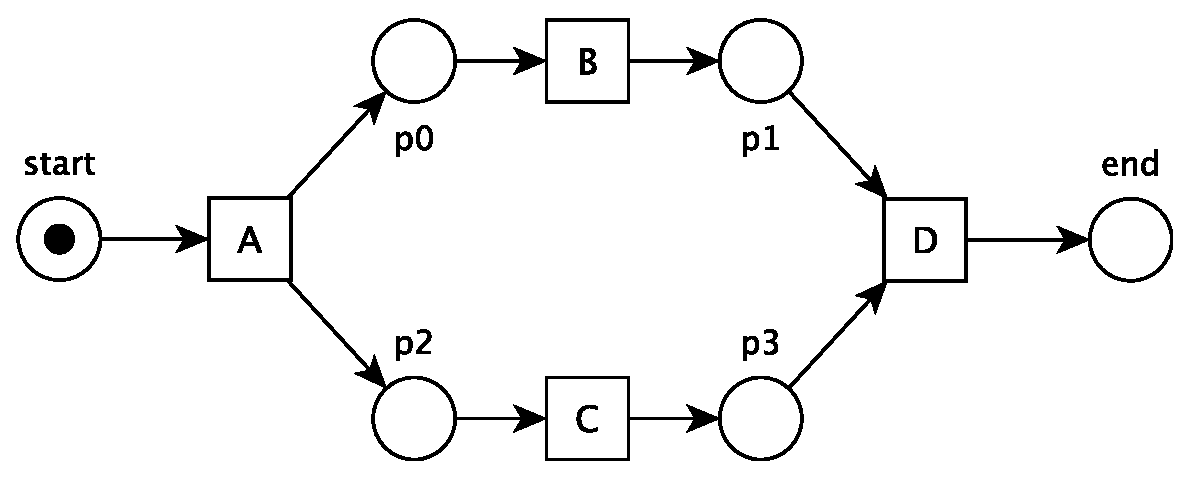
\includegraphics[scale=0.30]{./fig/LogReplay1a}
  \end{center}
  \begin {block}{Measures}
    \begin{tabular}{cc}
    \end{tabular}
  \end{block}
}
\frame{
  \begin{block}{Log-replay examples}
    Trace log $\alert{(A, 1s)}, (B, 2s), (C, 4s), (D, 8s)$ 
  \end{block}
  \begin{center}
    \includegraphics[scale=0.30]{./fig/LogReplay1b}
  \end{center}
  \begin {block}{Measures}
    \begin{tabular}{ccc}
                  & p0 & p2 \\
       $\TSync$   & 0  & 0  \\
    \end{tabular}
  \end{block}
}
\frame{
  \begin{block}{Log-replay examples}
    Trace log $(A, 1s), \alert{(B, 2s)}, (C, 4s), (D, 8s)$ 
  \end{block}
  \begin{center}
    \includegraphics[scale=0.30]{./fig/LogReplay1b}
  \end{center}
  \begin {block}{Measures}
    \begin{tabular}{ccc}
                  & p0 & p2 \\
       $\TSync$   & 0  & 0  \\
    \end{tabular}
  \end{block}
}
\frame{
  \begin{block}{Log-replay examples}
    Trace log $(A, 1s), \alert{(B, 2s)}, (C, 4s), (D, 8s)$ 
  \end{block}
  \begin{center}
    \includegraphics[scale=0.30]{./fig/LogReplay1c}
  \end{center}
  \begin {block}{Measures}
    \begin{tabular}{ccc}
                  & p0 & p2 \\
       $\TSync$   & 0  & 0  \\
       $\TTot$    & 1  &    \\
    \end{tabular}
  \end{block}
}
\frame{
  \begin{block}{Log-replay examples}
    Trace log $(A, 1s), (B, 2s), \alert{(C, 4s)}, (D, 8s)$ 
  \end{block}
  \begin{center}
    \includegraphics[scale=0.30]{./fig/LogReplay1c}
  \end{center}
  \begin {block}{Measures}
    \begin{tabular}{ccc}
                  & p0 & p2 \\
       $\TSync$   & 0  & 0  \\
       $\TTot$    & 1  &    \\
    \end{tabular}
  \end{block}
}
\frame{
  \begin{block}{Log-replay examples}
    Trace log $(A, 1s), (B, 2s), \alert{(C, 4s)}, (D, 8s)$ 
  \end{block}
  \begin{center}
    \includegraphics[scale=0.30]{./fig/LogReplay1d}
  \end{center}
  \begin {block}{Measures}
    \begin{tabular}{ccccccccc}
                  & p0 & p2 & p1 & p3 \\
       $\TSync$   & 0  & 0  & 2  & 0  \\
       $\TTot$    & 1  & 3  &    &    \\
    \end{tabular}
  \end{block}
}
\frame{
  \begin{block}{Log-replay examples}
    Trace log $(A, 1s), (B, 2s), (C, 4s), \alert{(D, 8s)}$ 
  \end{block}
  \begin{center}
    \includegraphics[scale=0.30]{./fig/LogReplay1d}
  \end{center}
  \begin {block}{Measures}
    \begin{tabular}{ccccccccc}
                  & p0 & p2 & p1 & p3 \\
       $\TSync$   & 0  & 0  & 2  & 0  \\
       $\TTot$    & 1  & 3  &    &    \\
    \end{tabular}
  \end{block}
}
\frame{
  \begin{block}{Log-replay examples}
    Trace log $(A, 1s), (B, 2s), (C, 4s), \alert{(D, 8s)}$ 
  \end{block}
  \begin{center}
    \includegraphics[scale=0.30]{./fig/LogReplay1e}
  \end{center}
  \begin {block}{Measures}
    \begin{tabular}{ccccccccc}
                  & p0 & p2 & p1 & p3 \\
       $\TSync$   & 0  & 0  & 2  & 0  \\
       $\TTot$    & 1  & 3  & 6  & 4  \\
    \end{tabular}
  \end{block}
}

%%% Local Variables: 
%%% mode: latex
%%% TeX-master: "main"
%%% End: 

\frame{
  \begin{block}{Log-replay examples}
    Trace log $(A, 1s), (B, 2s), (D, 8s)$ 
  \end{block}
  \begin{center}
    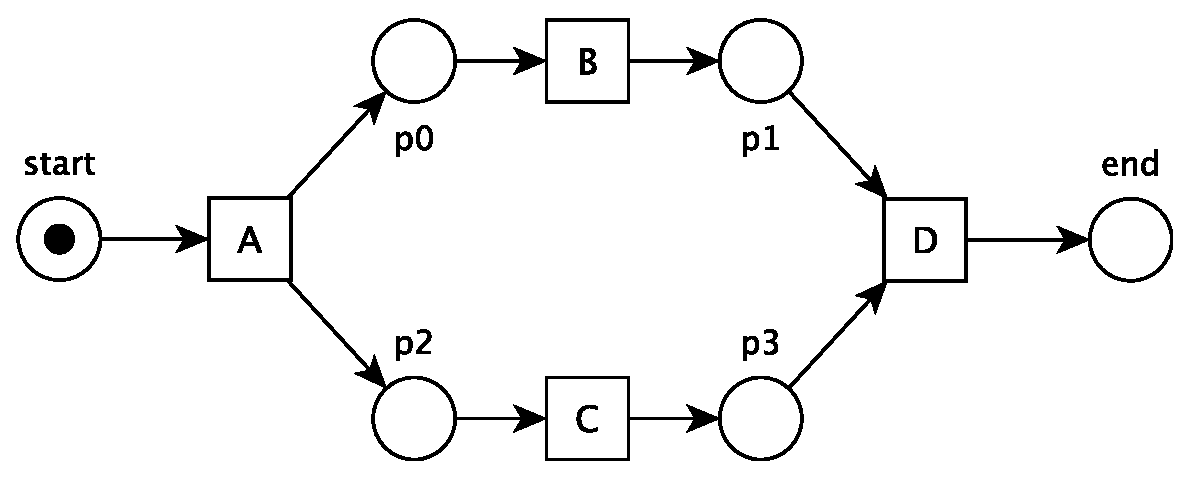
\includegraphics[scale=0.30]{./fig/LogReplay1a}
  \end{center}
  \begin {block}{Measures}
    \begin{tabular}{cc}
    \end{tabular}
  \end{block}
}
\frame{
  \begin{block}{Log-replay examples}
    Trace log $\alert{(A, 1s)}, (B, 2s), (D, 8s)$ 
  \end{block}
  \begin{center}
    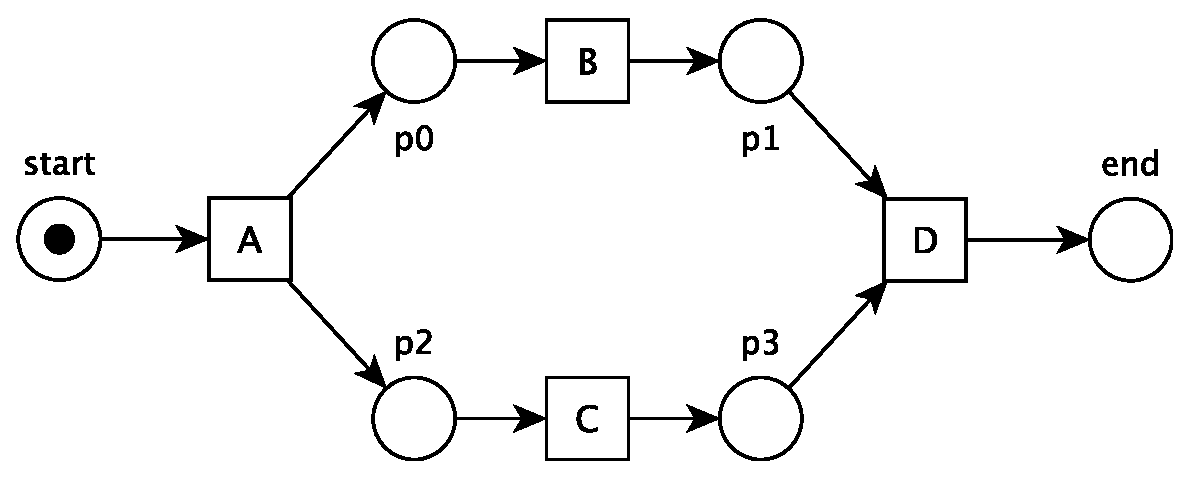
\includegraphics[scale=0.30]{./fig/LogReplay1a}
  \end{center}
  \begin {block}{Measures}
    \begin{tabular}{cc}
    \end{tabular}
  \end{block}
}
\frame{
  \begin{block}{Log-replay examples}
    Trace log $\alert{(A, 1s)}, (B, 2s), (D, 8s)$ 
  \end{block}
  \begin{center}
    \includegraphics[scale=0.30]{./fig/LogReplay1b}
  \end{center}
  \begin {block}{Measures}
    \begin{tabular}{ccc}
                  & p0 & p2 \\
       $\TSync$   & 0  & 0  \\
    \end{tabular}
  \end{block}
}
\frame{
  \begin{block}{Log-replay examples}
    Trace log $(A, 1s), \alert{(B, 2s)}, (D, 8s)$ 
  \end{block}
  \begin{center}
    \includegraphics[scale=0.30]{./fig/LogReplay1b}
  \end{center}
  \begin {block}{Measures}
    \begin{tabular}{ccc}
                  & p0 & p2 \\
       $\TSync$   & 0  & 0  \\
    \end{tabular}
  \end{block}
}
\frame{
  \begin{block}{Log-replay examples}
    Trace log $(A, 1s), \alert{(B, 2s)}, (D, 8s)$ 
  \end{block}
  \begin{center}
    \includegraphics[scale=0.30]{./fig/LogReplay1c}
  \end{center}
  \begin {block}{Measures}
    \begin{tabular}{ccc}
                  & p0 & p2 \\
       $\TSync$   & 0  & 0  \\
       $\TTot$    & 1  &    \\
    \end{tabular}
  \end{block}
}
\frame{
  \begin{block}{Log-replay examples}
    Trace log $(A, 1s), (B, 2s), \alert{(D, 8s)}$ 
  \end{block}
  \begin{center}
    \includegraphics[scale=0.30]{./fig/LogReplay1c}
  \end{center}
  \begin {block}{Measures}
    \begin{tabular}{ccc}
                  & p0 & p2 \\
       $\TSync$   & 0  & 0  \\
       $\TTot$    & 1  &    \\
    \end{tabular}
  \end{block}
}

\frame{
  \begin{block}{Log-replay examples}
    Trace log $(A, 1s), (B, 2s), \alert{(D, 8s)}$ 
  \end{block}
  \begin{center}
    \includegraphics[scale=0.30]{./fig/LogReplay2d}
  \end{center}
  \begin {block}{Measures}
    \begin{tabular}{ccc}
                  & p0 & p2 \\
       $\TSync$   & 0  & 0  \\
       $\TTot$    & 1  &    \\
    \end{tabular}
  \end{block}
}
\frame{
  \begin{block}{Log-replay examples}
    Trace log $(A, 1s), (B, 2s), \alert{(D, 8s)}$ 
  \end{block}
  \begin{center}
    \includegraphics[scale=0.30]{./fig/LogReplay2f}
  \end{center}
  \begin {block}{Measures}
    \begin{tabular}{ccc}
                  & p0 & p2 \\
       $\TSync$   & 0  & 0  \\
       $\TTot$    & 1  &    \\
    \end{tabular}
    \begin{tabular}{ccc}
                  & p3 \\
       $Missing$  & 1  \\
    \end{tabular}
  \end{block}
}
\frame{
  \begin{block}{Log-replay examples}
    Trace log $(A, 1s), (B, 2s), \alert{(D, 8s)}$ 
  \end{block}
  \begin{center}
    \includegraphics[scale=0.30]{./fig/LogReplay2g}
  \end{center}
  \begin {block}{Measures}
    \begin{tabular}{ccc}
                  & p0 & p2 \\
       $\TSync$   & 0  & 0  \\
       $\TTot$    & 1  &    \\
    \end{tabular}
    \begin{tabular}{ccc}
                  & p3 \\
       $Missing$  & 1  \\
    \end{tabular}
  \end{block}
}
\frame{
  \begin{block}{Log-replay examples}
    Trace log $(A, 1s), (B, 2s), \alert{(D, 8s)}$ 
  \end{block}
  \begin{center}
    \includegraphics[scale=0.30]{./fig/LogReplay2h}
  \end{center}
  \begin {block}{Measures}
    \begin{tabular}{ccc}
                  & p0 & p2 \\
       $\TSync$   & 0  & 0  \\
       $\TTot$    & 1  &    \\
    \end{tabular}
    \begin{tabular}{ccc}
                   & p3 & p2 \\
       $Missing$   & 1  & 0  \\
       $Remaining$ & 0  & 1   \\
    \end{tabular}
  \end{block}
}


%%% Local Variables: 
%%% mode: latex
%%% TeX-master: "main"
%%% End: 

% \frame{
  \begin{block}{Log-replay examples}
    Trace log $\alert{(A, 1s)}, (B, 2s), (C, 4), (D, 8s)$ 
  \end{block}
  \begin{center}
    \includegraphics[scale=0.30]{./fig/LogReplay3a}
  \end{center}
  \begin {block}{Measures}
    \begin{tabular}{ccc}
                  \\
       $\TSync$   \\
       $\TTot$    \\
    \end{tabular}
  \end{block}
}
\frame{
  \begin{block}{Log-replay examples}
    Trace log $\alert{(A, 1s)}, (B, 2s), (C, 4), (D, 8s)$ 
  \end{block}
  \begin{center}
    \includegraphics[scale=0.30]{./fig/LogReplay3b}
  \end{center}
  \begin {block}{Measures}
    \begin{tabular}{ccc}
                  & p0 & p2 \\
       $\TSync$   & 0  & 0  \\
       $\TTot$    &    &    \\
    \end{tabular}
  \end{block}
}
\frame{
  \begin{block}{Log-replay examples}
    Trace log $(A, 1s), \alert{(B, 2s)}, (C, 4), (D, 8s)$ 
  \end{block}
  \begin{center}
    \includegraphics[scale=0.30]{./fig/LogReplay3b}
  \end{center}
  \begin {block}{Measures}
    \begin{tabular}{ccc}
                  & p0 & p2 \\
       $\TSync$   & 0  & 0  \\
       $\TTot$    &    &    \\
    \end{tabular}
  \end{block}
}
\frame{
  \begin{block}{Log-replay examples}
    Trace log $(A, 1s), \alert{(B, 2s)}, (C, 4), (D, 8s)$ 
  \end{block}
  \begin{center}
    \includegraphics[scale=0.30]{./fig/LogReplay3c}
  \end{center}
  \begin {block}{Measures}
    \begin{tabular}{cccccc}
                  & p0 & p2 & p1 \\
       $\TSync$   & 0  & 0  & 0  \\
       $\TTot$    & 1  &    &    \\
    \end{tabular}
  \end{block}
}

% Attivazione di C
\frame{
  \begin{block}{Log-replay examples}
    Trace log $(A, 1s), (B, 2s), \alert{(C, 4)}, (D, 8s)$ 
  \end{block}
  \begin{center}
    \includegraphics[scale=0.30]{./fig/LogReplay3c}
  \end{center}
  \begin {block}{Measures}
    \begin{tabular}{cccccc}
                  & p0 & p2 & p1 \\
       $\TSync$   & 0  & 0  & 0  \\
       $\TTot$    & 1  &    &    \\
    \end{tabular}
  \end{block}
}
\frame{
  \begin{block}{Log-replay examples}
    Trace log $(A, 1s), (B, 2s), \alert{(C, 4)}, (D, 8s)$ 
  \end{block}
  \begin{center}
    \includegraphics[scale=0.30]{./fig/LogReplay3d}
  \end{center}
  \begin {block}{Measures}
    \begin{tabular}{cccccc}
                  & p0 & p2 & p1 & p3 \\
       $\TSync$   & 0  & 0  & 0  &    \\
       $\TTot$    & 1  & 3  &    &    \\
    \end{tabular}
  \end{block}
}

% attivazione D
\frame{
  \begin{block}{Log-replay examples}
    Trace log $(A, 1s), (B, 2s), (C, 4), \alert{(D, 8s)}$ 
  \end{block}
  \begin{center}
    \includegraphics[scale=0.30]{./fig/LogReplay3d}
  \end{center}
  \begin {block}{Measures}
    \begin{tabular}{cccccc}
                  & p0 & p2 & p1 & p3 \\
       $\TSync$   & 0  & 0  & 0  &    \\
       $\TTot$    & 1  & 3  &    &    \\
    \end{tabular}
  \end{block}
}
\frame{
  \begin{block}{Log-replay examples}
    Trace log $(A, 1s), (B, 2s), (C, 4), \alert{(D, 8s)}$ 
  \end{block}
  \begin{center}
    \includegraphics[scale=0.30]{./fig/LogReplay3e}
  \end{center}
  \begin {block}{Measures}
    \begin{tabular}{cccccc}
                  & p0 & p2 & p1 & p3 & p4 \\
       $\TSync$   & 0  & 0  & 0  & 4  & 0  \\
       $\TTot$    & 1  & 3  & 6  &    &   \\
    \end{tabular}
  \end{block}
}
\frame{
  \begin{block}{Log-replay examples}
    Trace log $(A, 1s), (B, 2s), (C, 4), \alert{(D, 8s)}$ 
  \end{block}
  \begin{center}
    \includegraphics[scale=0.30]{./fig/LogReplay3f}
  \end{center}
  \begin {block}{Measures}
    \begin{tabular}{cccccc}
                  & p0 & p2 & p1 & p3 & p4 \\
       $\TSync$   & 0  & 0  & 0  & 4  & 0  \\
       $\TTot$    & 1  & 3  & 6  & 4  & 0 \\
    \end{tabular}
  \end{block}
}

%%% Local Variables: 
%%% mode: latex
%%% TeX-master: "main"
%%% End: 


\subsection{A refined Performance analysis}
\frame{
  \begin{block}{A refined Performance analysis}
    \begin{itemize}
        \item Exploit standard log-replay techniques in order to reuse
          existing sw infrastructure
        \item Transform resulting transition list into eager sequences
    $R = [tr_1, .... , tr_n]$ for each $tr_i$ invisible transition
    \begin{itemize}
      \item let $tr_p$ the last preceding ($p < i$) visible transition
      \item $\bullet tr_i \cap tr_p \bullet  \not = \emptyset$
    \end{itemize}
    
    \item Straightforward algorithm: for each invisible transition $tr_i$
      
      \begin{enumerate}
        \item left shift the transition until a
          visible transition $\bullet tr_i \cap tr_p \bullet  \not =
          \emptyset$
          is found
      \end{enumerate}
      
    \item All conformance metrics are not changed

    \end{itemize}

  \end{block}

}

\frame{
  \begin{block}{Esempio Calcolo Performance}
    
    \begin{itemize}
      \item Eventi del log $(A, 1s), (B, 2s), (C, 4), (D, 8s)$ 
      \item Sequenza di transizioni del log replay  $A, B, C, t1, D$
      \item Risultato della sequenza \textquotedblleft eager\textquotedblright $A, B, t1, C, D$
    \end{itemize}

  \end{block}
  \begin{center}
    \includegraphics[scale=0.30]{./fig/LogReplay3a}
  \end{center}
  \begin {block}{Misure}
    \begin{tabular}{ccc}
                  \\
       $\TSync$   \\
       $\TTot$    \\
    \end{tabular}
  \end{block}
}

\frame{
  \begin{block}{Esempio Calcolo Performance}
    
    \begin{itemize}
      \item Eventi del log $\alert{(A, 1s)}, (B, 2s), (C, 4), (D, 8s)$ 
      \item Sequenza di transizioni del log replay  $A, B, C, t1, D$
      \item Risultato della sequenza \textquotedblleft eager\textquotedblright $\alert{A}, B, t1, C, D$
    \end{itemize}

  \end{block}
  \begin{center}
    \includegraphics[scale=0.30]{./fig/LogReplay3a}
  \end{center}
  \begin {block}{Misure}
    \begin{tabular}{ccc}
                  \\
       $\TSync$   \\
       $\TTot$    \\
    \end{tabular}
  \end{block}
}

\frame{
  \begin{block}{Esempio Calcolo Performance}
    
    \begin{itemize}
      \item Eventi del log $\alert{(A, 1s)}, (B, 2s), (C, 4), (D, 8s)$ 
      \item Sequenza di transizioni del log replay  $A, B, C, t1, D$
      \item Risultato della sequenza \textquotedblleft eager\textquotedblright $\alert{A}, B, t1, C, D$
    \end{itemize}

  \end{block}
  \begin{center}
    \includegraphics[scale=0.30]{./fig/LogReplay3b}
  \end{center}
  \begin {block}{Misure}
    \begin{tabular}{ccc}
                  & p0 & p2 \\
       $\TSync$   & 0  & 0  \\
       $\TTot$    &    &    \\
    \end{tabular}
  \end{block}
}
\frame{
  \begin{block}{Esempio Calcolo Performance}
    
    \begin{itemize}
      \item Eventi del log $(A, 1s), \alert{(B, 2s)}, (C, 4), (D, 8s)$ 
      \item Sequenza di transizioni del log replay  $A, B, C, t1, D$
      \item Risultato della sequenza \textquotedblleft eager\textquotedblright $A, \alert{B}, t1, C, D$
    \end{itemize}

  \end{block}
  \begin{center}
    \includegraphics[scale=0.30]{./fig/LogReplay3b}
  \end{center}
  \begin {block}{Misure}
    \begin{tabular}{ccc}
                  & p0 & p2 \\
       $\TSync$   & 0  & 0  \\
       $\TTot$    &    &    \\
    \end{tabular}
  \end{block}
}
\frame{
  \begin{block}{Esempio Calcolo Performance}
    
    \begin{itemize}
      \item Eventi del log $(A, 1s), \alert{(B, 2s)}, (C, 4), (D, 8s)$ 
      \item Sequenza di transizioni del log replay  $A, B, C, t1, D$
      \item Risultato della sequenza \textquotedblleft eager\textquotedblright $A, \alert{B}, t1, C, D$
    \end{itemize}

  \end{block}
  \begin{center}
    \includegraphics[scale=0.30]{./fig/LogReplay3c}
  \end{center}
  \begin {block}{Misure}
    \begin{tabular}{cccccc}
                  & p0 & p2 & p1 \\
       $\TSync$   & 0  & 0  & 0  \\
       $\TTot$    & 1  &    &    \\
    \end{tabular}
  \end{block}
}

% Attivazione di t1
\frame{
  \begin{block}{Esempio Calcolo Performance}
    
    \begin{itemize}
      \item Eventi del log $(A, 1s), \alert{(B, 2s)}, (C, 4), (D, 8s)$ 
      \item Sequenza di transizioni del log replay  $A, B, C, t1, D$
      \item Risultato della sequenza \textquotedblleft eager\textquotedblright $A, B, \alert{t1}, C, D$
    \end{itemize}

  \end{block}
  \begin{center}
    \includegraphics[scale=0.30]{./fig/LogReplay3c}
  \end{center}
  \begin {block}{Misure}
    \begin{tabular}{cccccc}
                  & p0 & p2 & p1 \\
       $\TSync$   & 0  & 0  & 0  \\
       $\TTot$    & 1  &    &    \\
    \end{tabular}
  \end{block}
}
\frame{
  \begin{block}{Esempio Calcolo Performance}
    
    \begin{itemize}
      \item Eventi del log $(A, 1s), \alert{(B, 2s)}, (C, 4), (D, 8s)$ 
      \item Sequenza di transizioni del log replay  $A, B, C, t1, D$
      \item Risultato della sequenza \textquotedblleft eager\textquotedblright $A, B, \alert{t1}, C, D$
    \end{itemize}
  \end {block}
  \begin{center}
    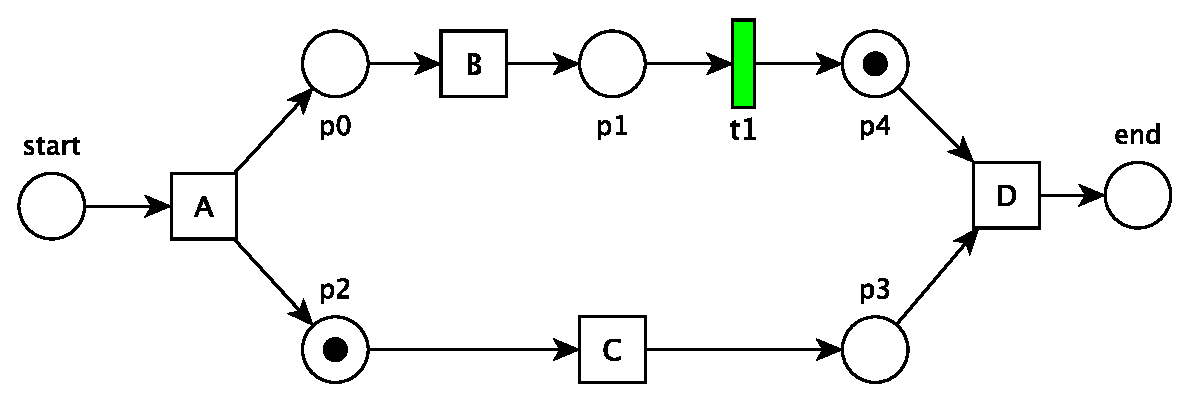
\includegraphics[scale=0.30]{./fig/LogReplay4d}
  \end{center}
  \begin {block}{Misure}
    \begin{tabular}{cccccc}
                  & p0 & p2 & p1 & p3 & p4 \\
       $\TSync$   & 0  & 0  & 0  &    &    \\
       $\TTot$    & 1  &    & 0  &    &    \\
    \end{tabular}
  \end{block}
}

\frame{
  \begin{block}{Esempio Calcolo Performance}
    
    \begin{itemize}
      \item Eventi del log $(A, 1s), (B, 2s), \alert{(C, 4)}, (D, 8s)$ 
      \item Sequenza di transizioni del log replay  $A, B, C, t1, D$
      \item Risultato della sequenza \textquotedblleft eager\textquotedblright $A, B, t1, \alert{C}, D$
    \end{itemize}
  \end {block}
  \begin{center}
    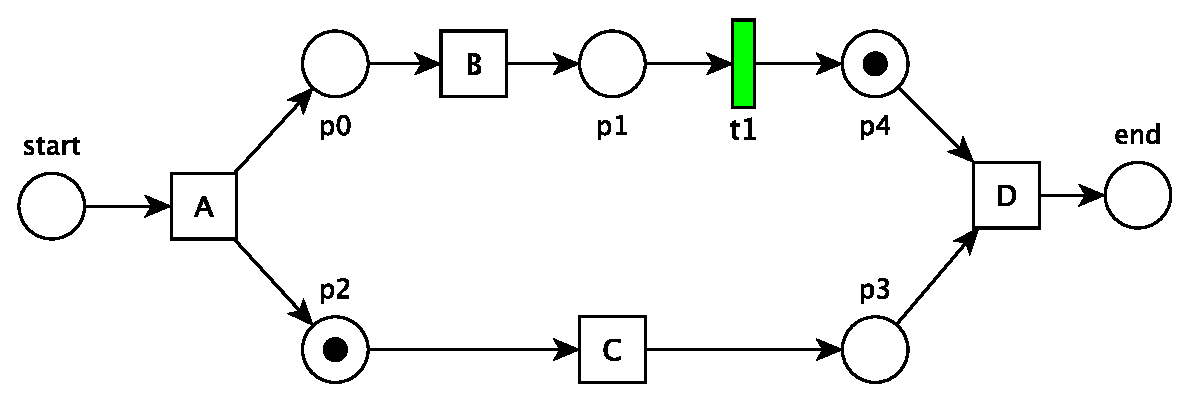
\includegraphics[scale=0.30]{./fig/LogReplay4d}
  \end{center}
  \begin {block}{Misure}
    \begin{tabular}{cccccc}
                  & p0 & p2 & p1 & p3 & p4 \\
       $\TSync$   & 0  & 0  & 0  &    &    \\
       $\TTot$    & 1  &    & 0  &    &    \\
    \end{tabular}
  \end{block}
}
\frame{
  \begin{block}{Esempio Calcolo Performance}
    
    \begin{itemize}
      \item Eventi del log $(A, 1s), (B, 2s), \alert{(C, 4)}, (D, 8s)$ 
      \item Sequenza di transizioni del log replay  $A, B, C, t1, D$
      \item Risultato della sequenza \textquotedblleft eager\textquotedblright $A, B, t1, \alert{C}, D$
    \end{itemize}
  \end {block}
  \begin{center}
    \includegraphics[scale=0.30]{./fig/LogReplay4e}
  \end{center}
  \begin {block}{Misure}
    \begin{tabular}{cccccc}
                  & p0 & p2 & p1 & p3 & p4 \\
       $\TSync$   & 0  & 0  & 0  & 0  & 2  \\
       $\TTot$    & 1  & 2  & 0  &    &    \\
    \end{tabular}
  \end{block}
}
\frame{
  \begin{block}{Esempio Calcolo Performance}
    
    \begin{itemize}
      \item Eventi del log $(A, 1s), (B, 2s), (C, 4), \alert{(D, 8s)}$ 
      \item Sequenza di transizioni del log replay  $A, B, C, t1, D$
      \item Risultato della sequenza \textquotedblleft eager\textquotedblright $A, B, t1, C, \alert{D}$
    \end{itemize}
  \end {block}
  \begin{center}
    \includegraphics[scale=0.30]{./fig/LogReplay4e}
  \end{center}
  \begin {block}{Misure}
    \begin{tabular}{cccccc}
                  & p0 & p2 & p1 & p3 & p4 \\
       $\TSync$   & 0  & 0  & 0  & 0  & 2  \\
       $\TTot$    & 1  & 2  & 0  &   &   \\
    \end{tabular}
  \end{block}
}
\frame{
  \begin{block}{Esempio Calcolo Performance}
    
    \begin{itemize}
      \item Eventi del log $(A, 1s), (B, 2s), (C, 4), \alert{(D, 8s)}$ 
      \item Sequenza di transizioni del log replay  $A, B, C, t1, D$
      \item Risultato della sequenza \textquotedblleft eager\textquotedblright $A, B, t1, C, \alert{D}$
    \end{itemize}
  \end {block}
  \begin{center}
    \includegraphics[scale=0.30]{./fig/LogReplay4f}
  \end{center}
  \begin {block}{Misure}
    \begin{tabular}{cccccc}
                  & p0 & p2 & p1 & p3 & p4 \\
       $\TSync$   & 0  & 0  & 0  & 0  & 2  \\
       $\TTot$    & 1  & 2  & 0  & 4  & 6  \\
    \end{tabular}
  \end{block}
}
%%% Local Variables: 
%%% mode: latex
%%% TeX-master: "main"
%%% End: 


\frame{
  Example of conformance analysis
  \begin{center}
    \includegraphics[scale=0.50]{./fig/ConfPN}\\[10pt]
    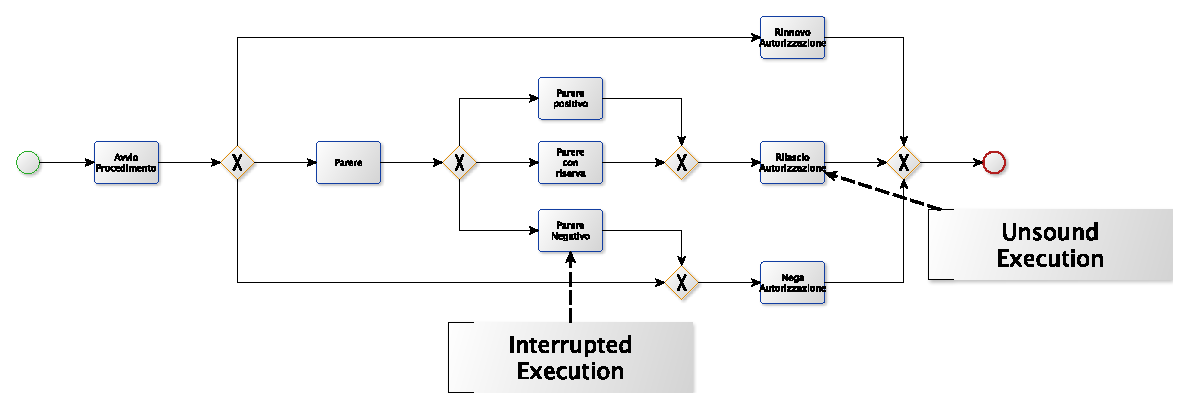
\includegraphics[scale=0.50]{./fig/BPMNConf}
  \end{center}

}
\section{From Analysis to BPMN}
\frame{
  \begin{block}{From Analysis to BPMN (Conformance)}
    \begin{itemize}
      \item \alert{Missing tokens}: Log replay produces missing tokens only to fire
        visible transitions $\Rightarrow$ pre-set of at least one visible
        transition
      \item \alert{Remaining tokens} fires invisible transitions fired
        only if  required by visible transition $\Rightarrow$ 
        places in the post-set of a visible transition or of an invisible
transition spawning several tokens

    \end{itemize}
  \end{block}
  
  \begin{center}
    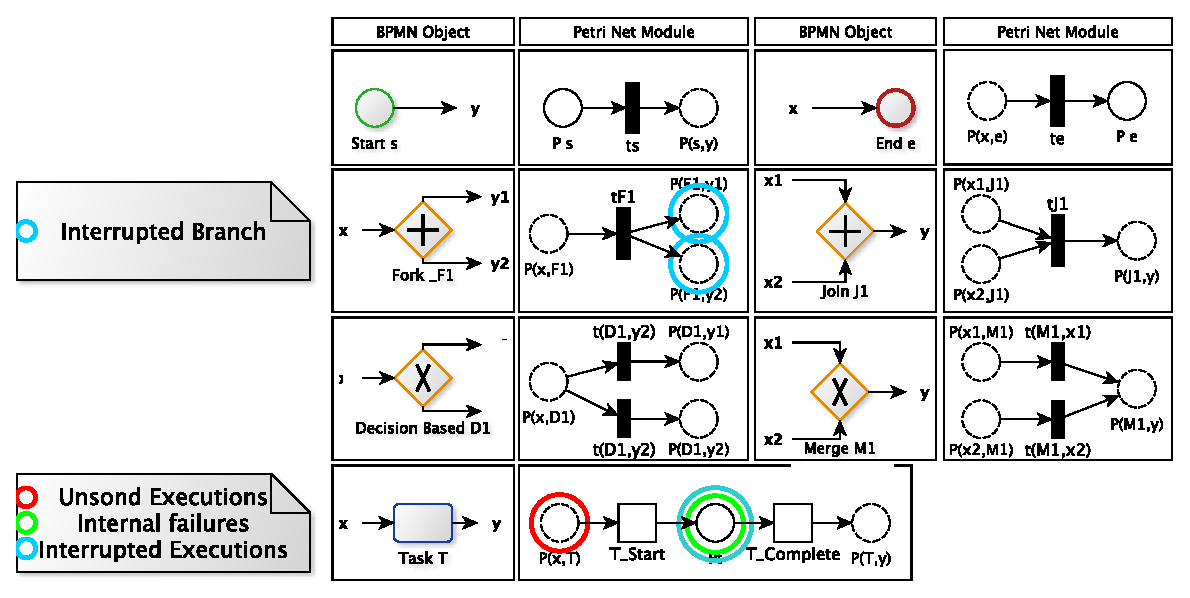
\includegraphics[scale=0.40]{./fig/MappingBPMNtoPN2}
  \end{center}

}

\frame{
  Example of performance analysis
  \begin{center}
    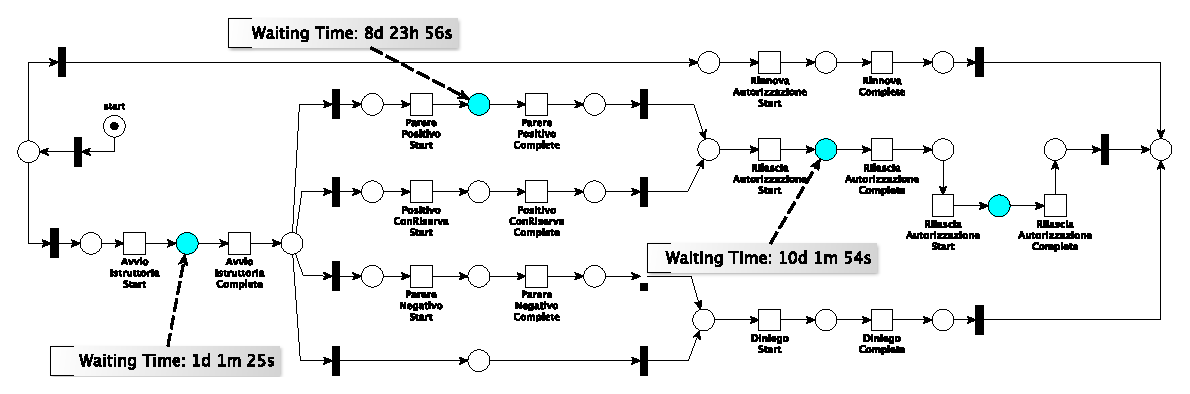
\includegraphics[scale=0.55]{./fig/PerfPN}\\[10pt]
    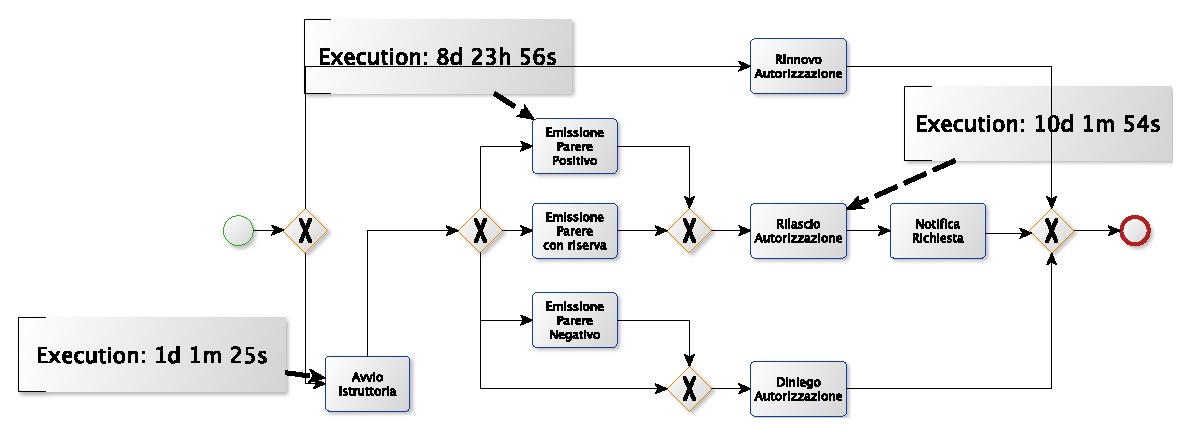
\includegraphics[scale=0.50]{./fig/BPMNPerf}
  \end{center}
}

\frame{
  \begin{block}{From Analysis to BPMN (Performance)}
    \begin{itemize}
      \item \alert{Waiting time}: invisible transitions fired
        immediately $\Rightarrow$ pre-set of visible transitions
      \item \alert{Synchronization time} places having at least one
transition in their post-set that depends on another place.
    \end{itemize}
  \end{block}
  
  \begin{center}
    \includegraphics[scale=0.50]{./fig/MappingBPMNtoPN3}
  \end{center}

}

\section{Concluding Remarks}
\frame{
  \begin{block}{June results}
    \begin{itemize}
      \item Refined PetriNet techniques to handle invisible
        transitions
      \item Methodology to project measures on the BPMN model
      \item A new ProM context to execute the plug-ins into a GUI-less
      environment
    \item Eager Sequence transformer plug-in
    \item PetriNet performance evaluator plug-in
    \end{itemize}
  \end{block}
  \begin{block}{Current results}
    \begin{itemize}
        \item Model transformation from BPMN to PetriNet plug-in
        \item Projection of PetriNet measures to the starting BPMN
          model plug-in
    \end{itemize}
  \end{block}
  \begin{block}{Ongoing works}
    \begin{itemize}
    \item Extensions to the BPMN management to handle task life-cycle
      and intermediate events
    \item Integration of DataMining tool-kits
    \end{itemize}
  \end{block}
}
\frame{\tableofcontents}

\end{document}


%%% Local Variables: 
%%% mode: latex
%%% TeX-master: t
%%% End: 
